\subsection{自由连接链模型}
\begin{figure}
				\caption{ }
				\centering
				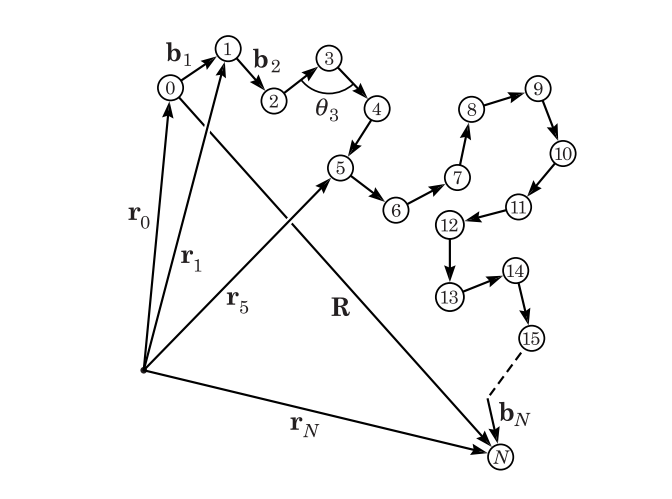
\includegraphics[width=9cm]{./figures/2-1.png}
			\end{figure}
对于一般含$N+1$个粒子的粗粒聚合物模型,如图2.1所示,单个链的构象配分函数(配分函数是一个平衡态统计物理学中经常应用到的概念,经由计算配分函数可以将微观物理状态与宏观物理量相互联系起来,而配分函数等价于自由能,与路径积分在数学上有巧妙的类似。)可以用类似$Z=\int dr^{N+1}exp[-\beta U(r^{n})]$(1.6)的表示:\\
\begin{gather}
Z_0 = \int dr^{N+1}exp[-\beta U_{0}(r^{N+1})]
\end{gather}
其中$r^{N+1}=(r_0,r_1,\ldots,r_{N})$表示$N+1$粒子的位置,$U_0(r^{N+1})$是与聚合物特定构型相关联的势能(下标$0$用来表示我们正在讨论单个理想链的性质)。$\int dr^{N+1}$是三维区域内$N+1$粒子所占体积积分的缩写。对于理想链模型,$U_0$只包含反映短程干扰的相互作用势项。\\

在构象空间中观测点$r^{N+1}$的联合概率密度是波尔兹曼(Boltzmann)分布(也叫吉布斯分布,是一种覆盖系统各种状态的概率分布、概率测量或者频率分布。当有保守外力(如重力场、电场等)作用时,气体分子的空间位置就不再均匀分布了,不同位置处分子数密度不同。玻尔兹曼分布律是描述理想气体在受保守外力作用、或保守外力场的作用不可忽略时,处于热平衡态下的气体分子按能量的分布规律):\\
\begin{gather}
P_0(r^{N+1})=Z_{0}^{-1}exp[[-\beta U_{0}(r^{N+1})]
\end{gather}
此概率权重(或密度)被规范化,以便$\int dr^{N+1}p_0(r^{N+1})=1$。在链的所有配置上,任意函数$f(r^{N+1})$的系综平均值可以写成\\
\begin{gather}
\langle f(r^{N+1})\rangle _0 =  \int dr^{N+1}P_0(r^{N+1})f(r^{N+1})
\end{gather}
另一种表示$N+1$粒子链构象自由度的方法是保留一个描述聚合物整体位置的“外部”坐标和N个“内部”坐标。一个特别方便的选择是链端的位置,例如,以及图2.1所示的N 个键向量,$b^{N}=(b_1,b_2,\ldots,b_{N})$,其中$b_{i}=r_{i}-r_{i-1}$。在聚合物没有外部势作用的情况下,$U_0$只依赖于内部坐标$b^{N}$。将$r^{N+1}$和$(r_0,b^{N})$ 进行雅克比变换,(1)–(2) 可重新表示为\\
\begin{gather}
Z_0 = V \int db^{N}exp[-\beta U_{0}(b^{N})]
\end{gather}
\begin{gather}
P_0(r_0,b^{N})=Z_{0}^{-1}exp[[-\beta U_{0}(b^{N})]
\end{gather}
因此,在链端位置$r_0$分布是均匀的。\\

自由连接链模型是一种非常简单的理想链模型,其中连接连续粒子的键向量被约束为一个固定的长度,$|b_{i}|=b$,但N个键向量的方向是各向同性独立分布的。在无限刚性弹簧的极限情况下,$U_0(b^{N})$的弹簧模型原则上可以实现固定键长的约束。一个更简单的方法是采用一个$b^{N}$表示法,这样约束就会自动得到满足。另$b_{i}=bn_{i}$,其中$n^{N}=(n_1,n_2,\ldots,n_{N})$是单位球面上一组均匀独立分布的N个单位向量。因此,对于自由连接链模型\\
\begin{gather}
P_0(r_0,n^{N})=\frac{1}{V} (\frac{1}{4 \pi})^{N}
\end{gather}
它是规范化的,所以$\int dr_0\int dn^{N}P_0(r_0,n^{N})=1$,其中$\int dn^{N}$表示单位球面上的N个积分。\\
应用上式,我们可以检验自由连接链的各种统计性质。特别是端到端向量$R=r_{N}-r_0$的矩,还可以写为$R=\sum _{i=1}^{N} b_{i}=b \sum _{i=1}^{N} n_{i}$.
$n_{i}$的各向同性分布意味着$\langle n_{i}\rangle _{0}=0$,因此R的一阶矩消失\\
\begin{gather}
\langle R \rangle_{0}=0
\end{gather}
端到端的二阶矩可以写出来\\
\begin{gather}
\langle R_{\alpha} R_{\beta}\rangle_{0}=b^2 \sum _{i=1}^{N} \sum _{j=1}^{N} \langle n_{i \alpha},n_{j \beta} \rangle_{0}
\end{gather}
这里我们用希腊下标来表示向量和张量的笛卡尔分量。当$i\neq j$双和项由于各单位向量的独立性而明显消失。对角线项用$\langle n_{i \alpha},n_{j \beta} \rangle_{0}=(1/3)\delta_{\alpha  \beta }$计算,其中$\delta_{\alpha \beta }$是克罗内克(Kronecker)符号,因此:\\
\begin{gather}
\langle R_{\alpha} R_{\beta}\rangle_{0}=\frac{b^{2}N}{3}\delta_{\alpha \beta }
\end{gather}
所以自由连接链模型的均方端到端向量完全符合理想链标度定律$R~bN^2,\nu=1/2,N \rightarrow \infty $(2.1):\\
\begin{gather}
R\equiv \sqrt{\langle R \cdot R\rangle _{0}}=bN^{1/2}
\end{gather}
注意,上式是在不施加$N\rightarrow \infty$的情况下导出的,(2.1)中省略的标度系数对于自由连接链是完全统一的。\\

端到端向量的更高矩也可以同样计算出来。例如\\
\begin{gather}
\langle (R \cdot R)^2 \rangle_{0}=\frac{5}{3}b^4N(N-\frac{2}{5})
\end{gather}
从这个结果可以看出,自由连接链的端到端向量R的概率分布不是简单的高斯分布,因为对于这种分布(见附录B)$\langle (R \cdot R)^2 \rangle=\langle (R \cdot R) \rangle^2+2\langle (R R)\rangle:\langle (R R)\rangle$,这导致$\langle (R \cdot R)^2 \rangle_{0}=(5/3)b^4N^2$。但是,对于$N\rightarrow \infty$,上式中给出的四阶矩与高斯分布是一致的。\\

衡量聚合物链平均尺寸的另一个重要指标是回转半径$R_{g}$。这个量是单个片段(粒子)与聚合物质心之间的均方距离,$R_{c}=(N+1)^{-1} \sum _{i=0}^{N} r_{i}$,即\\
\begin{gather}
R_{g}^2 \equiv \frac{1}{N+1} \sum _{i=0}^{N} \langle (r_{i}- R_{c})^2 \rangle_{0} 
\end{gather}
因此$R_{G}^2$代表了质量分布在聚合物线圈中的二阶矩,而且还可以定义为所有聚合物的结构,例如没有链端的环状聚合物。旋转的平方半径可由另一种形式表示\\
\begin{gather}
R_{g}^2=\frac{1}{(N+1)^2} \sum _{i=0}^{N} \sum _{j>i}^{N} \langle (r_{i}- r_{j})^2 \rangle_{0} 
\end{gather}
这公式特别容易计算。还可以通过将$r_{i}-r_{j}$表示为键向量之和来计算自由连接链的表达式,从而得到$\langle (r_{i}- r_{j})^2 \rangle_{0}=b^2 |i-j|$。然后对上式中的二重和进行渐近求和,使$N \rightarrow \infty $。\\
\begin{gather}
R_{g} \approx b(N/6)^{1/2}
\end{gather}
因此,自由连接链的回转半径比均方端到端向量R小$1/\sqrt{6}$。这证明了在N足够大时线性聚合物的任何理想链模型都是成立的。\\
\begin{figure}
				\caption{ }
				\centering
				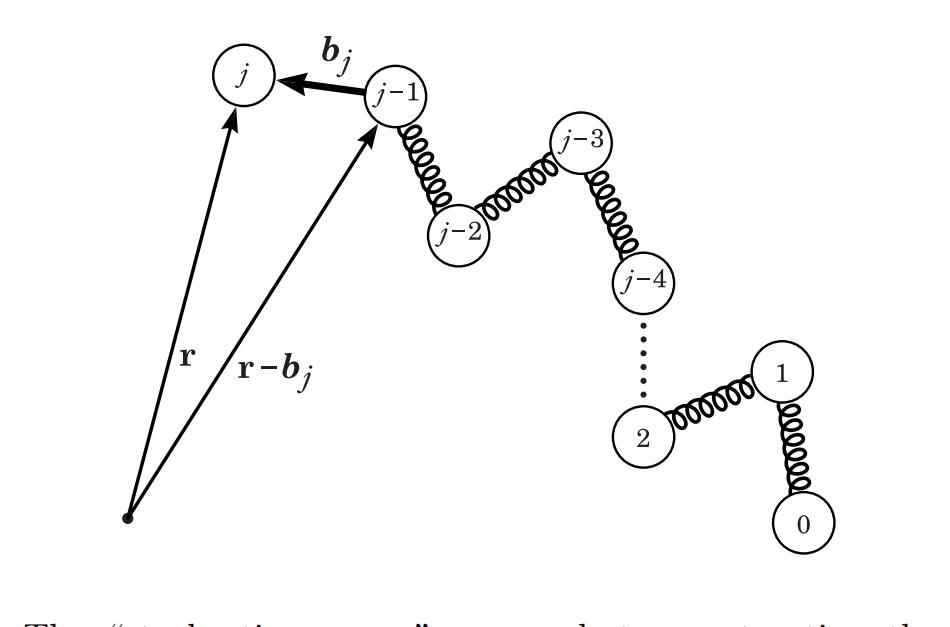
\includegraphics[width=9cm]{./figures/3.png}
			\end{figure}
图2.2从j个粒子链的统计权重出发,用“随机过程”方法建立具有j+1粒子的自由连接链末端位置的统计权重。\\

另一种探索理想链模型统计特性的方法不是计算矩,而是直接检测诸如端到端向量等量的概率分布函数。特别是约化分布函数$p_{0}(r,j)$,它表示含有$j+1$个粒子的聚合物链在其末端r位置(粒子标记的j)的概率密度。该函数被规范化,以便$\int drp_0(r,j)=1$。在构造这一目标时,我们将有机会在聚合物统计力学与随机过程理论之间建立一个重要的联系。具体来说,连续粒子沿粗粒聚合物链的随机位移类似于离散时间随机过程中在一定时间间隔内发生的随机事件。\\

为了利用随机过程的类比,我们假设一个含有较少粒子的链的末端$p_{0}(r,j-1)$的概率密度是已知的,如图2.2所示,一个$(j+1)$粒子链可以通过添加一个粒子和一个连接键从j粒子链中建立。在自由连接链模型中,附加键的长度是固定的,但它的取向与链中已经存在的$j−1$个键的方向无关。因此,我们可以从已知的函数$p_{0}(r,j)$乘以一个跃迁概率(与所加键的固定长度和均匀方向分布一致)求出概率密度,并对所有可能的键方向进行积分,\\
\begin{gather}
p_{0}(r,j)=\frac{1}{4 \pi} \int dnp_0(t-bn,j-1)
\end{gather}
这个方程中的因子$1/(4 \pi)$表示与所加键的取向有关的均匀跃迁概率,积分又在单位球面上。这种方程在随机过程理论中称为查普曼-科莫高洛夫(Chapman-Kolmogorov)方程。在这里,自由连接链是一步马尔可夫过程的一个例子,因为跃迁概率只连接链上相邻的粒子。\\

对于解像$(15)$这样的方程,我们需要一个“初始条件”,指定一个1-粒子链的位置分布。然后依次迭代求出$(N+1)$-粒子链末端位置的概率密度$p_{0}(r,N)$,这种递推格式非常适合于数值计算。就目前的目的而言,$(15)$可用于推导自由连接链的端到端向量的全部分布函数。\\

为了方便,引入函数$f(R)$的三维傅里叶变换(与傅里叶分析有关的定义和公式在附录A中)\\
\begin{gather}
\hat{f}(k)=\int dre^{-ik \cdot r}f(r)
\end{gather}
给出逆变换\\
\begin{gather}
 f(r)=\frac{1}{(2 \pi)^3} \int dke^{ik \cdot r} \hat{f}(k)
\end{gather}
将傅里叶变换应用于$(15)$的两边,得到以下表达式:\\
\begin{gather}
\hat{p_0}(k,j)=\frac{1}{4 \pi} \int dne^{-ibk \cdot n} \hat{p_0}(k,j-1)=j_0(b|k|)\hat{p_0}(k,j-1)
\end{gather}
其中$j_0(x) \equiv (sinx)/x$是常见的球面贝塞尔函数。依次地将这个方程应用于$j=1,2,\ldots,N$得到\\
\begin{gather}
\hat{p_0}(k,N)=[j_0(b|k|)]^{N}\hat{p_0}(k,0)
\end{gather}
特别有趣的情形是对应于初始条件$p_0(r,0)=\delta(r)$,其中$\delta(r)$是三维狄拉克函数(狄拉克函数是由性质定义的广义函数,对于任何函数成立,另见附录A)。这意味着链的起始端(粒子$0$) 被约束于原点。有了这种选择,$\hat{p_0}(k,0)=1$,$p_0(R,N)$可以解释为含有N个键和端到端向量的自由连接链的概率密度。因此\\
\begin{gather}
p_0(R,N)=\frac{1}{(2 \pi)^3 }\int dke^{ik \cdot R}[j_0(b|k|)]^{N}
\end{gather}
是端到端向量的概率密度的精确闭型表达式。当$N\gg1$且$|R| \ll Nb $时,对这个积分的渐近分析证实了我们先前观察到的R的二阶和四阶矩与高斯分布是一致的。\\
\begin{gather}
p_0(R,N) \approx [3/(2 \pi Nb)]^{3/2}exp[-3|R|^2/(2Nb^2)]
\end{gather}
构象熵的重要概念体现在上式中。在自由连接链的全相空间分布函数$P_0(r_0,b^{N})$与端到端向量的约化概率分布函数$p_0(R,N)$转换的过程中,我们固定端到端向量$R=\sum _{i=1}^{N} b_{i}$,在所有固定长度键向量b 上进行了积分。这种集成相当于对构象状态的枚举。由于在自由连接的模型中,所有的状态都以均匀的概率发生,所以结果是对约束端到端向量R 的链的自由能的纯粹熵表现:\\
\begin{gather}
F_0(R)=-k_{B}Tlnp_0(R,N)\approx \frac{3k_{B}T}{2Nb^2}|R|^2
\end{gather}
这个表达式中的二次项依赖于链的扩张维R可以看作是一个“熵弹簧”势。对于具有较大扩展的链,可用的构象态较少,因此自由能随的增加而增加。此外,$\frac{3k_{B}T}{Nb^2}=\frac{k_{B}T}{2R^2_{g}}$的“弹簧常数”与聚合物线圈尺寸的平方成反比。\\

最后一个主题涉及到自由连接链模型在理想条件下对真实链的适用性。在短尺度(约$1nm$)上,自由连接链明显地简化了真实聚合物链的键合和空间约束,该链仅在一定距离b上包含局部键刚性。然而,在较大的尺度上,即$5~10nm$,真实的柔性聚合物在理想状态下表现出符合$(10)$的自由连接链的标度行为。因此,我们可以通过定义一个等效的自由连接链来描述这类聚合物的介观统计特性。即要求处于理想状态的真实聚合物具有相同的均方端到端向量$R^2=Nb^2$,最大端到端距离$R_{max}=Nb$作为等效的自由连接链。然后,自由连接链的两个参数可以用实验测量或$R^2=\langle R \cdot R\rangle_{0}$和$R_{max}$的估计来表示\\
\begin{gather}
b=R^2/R_{max},N=R_{max}^{2}/R^2
\end{gather}
按照这一程序,等价链的键长b称为库恩段长度,对大多数乙烯基聚合物而言约为$1nm$。等价链的有效“库恩段”的个数N通常比实际链的骨架键数小$50$倍。\\

显然,$(23)$中给出的将理想状态下的真实链映射到自由连接模型上的条件并不是唯一的。高度扩展的链构象是非常罕见的,因此在实链和等价链之间匹配$R_{max}$的理由是很弱的。定义等效自由连接链的其他方法通常涉及N的定义,然后通过匹配实链和等价链之间的$R^2$(或$R_{g}^{2}$)来计算b。N的一般定义包括每条链的单体重复单位的平均数目,或每条具有规定分子量的链段的平均数目(这可能与实际的化学重复单位相对应,也可能不对应)。从这些过程中获得的b值通常称为统计段长度。需要注意的是,b 和N的值将因定义等价链所用的标准而有所不同。然而,所建立的链模型一般都能很好地描述真实聚合物链在理想状态下的介观$(1nm)$统计特性,而不考虑所应用的准则。\\

在本专著中,我们将采用一种比较随意的语言来引用粗粒度、等价链模型中的参数。n将可互换地描述为聚合度、每个链的单体数或统计段数。同样,b将被称为库恩长度,统计段长度,或单体长度。\\
\endinput
